%%%%%%%%%%%%%%%%%%%%%%%%%%%%%%%%%%%%%%%%%%%%%%%%%%%%%%%%%%%%%%%%%%%%%%%%%%%%%%%
% Title: UTDesign Report Template
% Author: Daanish Khazi-Syed
% Date: 2020-05-26
%%%%%%%%%%%%%%%%%%%%%%%%%%%%%%%%%%%%%%%%%%%%%%%%%%%%%%%%%%%%%%%%%%%%%%%%%%%%%%%

% Preamble
%%%%%%%%%%%%%%%%%%%%%%%%%%%%%%%%%%%%%%%%%%%%%%%%%%%%%%%%%%%%%%%%%%%%%%%%%%%%%%%
\documentclass[12pt]{article}
\usepackage[utf8]{inputenc}
\usepackage[T1]{fontenc}
\usepackage[letterpaper, margin=1in]{geometry}
\usepackage{microtype}
\usepackage{newtxtext, newtxmath}
\usepackage{enumitem}
\usepackage{booktabs}
\usepackage{lipsum}  % Generates filler text

\usepackage{float, graphicx}
\graphicspath{ {figures/} }
\usepackage{caption, subcaption}

\usepackage{listings}

\usepackage[style=ieee]{biblatex}
\addbibresource{references.bib}

\usepackage[toc, page]{appendix}
\usepackage[titles]{tocloft}
\renewcommand{\cftsecleader}{\cftdotfill{\cftdotsep}}

\usepackage{fancyhdr, lastpage}
\pagestyle{fancy}
\fancyhead{}
\fancyfoot[c]{ Page \thepage\ of \pageref{LastPage} }
\renewcommand{\headrulewidth}{0pt}

\usepackage{pdflscape}
\def\lscapefooter{
    \par\pagestyle{empty}
    % \vbox to 0pt{\vss}
    % \vfill
    \vbox to 0pt{
        \baselineskip0pt
        \hbox to\linewidth{\hss}
        \baselineskip\footskip
        \hbox to\linewidth{\hfill Page \thepage\ of \pageref{LastPage} \hfill}
        \vss
    }
}

\usepackage{parskip, setspace}
\setstretch{1.15}
\setlength{\parindent}{0pt}
\setlength{\jot}{18pt}

\usepackage{hyperref}
\hypersetup{
    colorlinks=true,
    anchorcolor=black,
    citecolor=black,
    filecolor=black,
    linkcolor=black,
    urlcolor=blue,
    bookmarksopen=true,
}
\urlstyle{same}

% Edit these document details
\newcommand{\Title}{Report}
\newcommand{\Date}{26 August 2019}

\renewcommand{\contentsname}{Table of Contents}
%%%%%%%%%%%%%%%%%%%%%%%%%%%%%%%%%%%%%%%%%%%%%%%%%%%%%%%%%%%%%%%%%%%%%%%%%%%%%%%

\begin{document}

% Cover Page (edit [details] listed in square brackets)
%%%%%%%%%%%%%%%%%%%%%%%%%%%%%%%%%%%%%%%%%%%%%%%%%%%%%%%%%%%%%%%%%%%%%%%%%%%%%%%
\thispagestyle{empty}
\pdfbookmark[1]{Cover Page}{Cover Page}
\begin{center}
    
\includegraphics[width=3.5in]{figures/team_logo.png} \\
    \vspace{6pt}
    
\includegraphics[width=3.5in]{figures/utdesign_logo.png} \\
    \vspace{0.75in}
    \Large
    Project No. XXX: [Project Name] \\
    Corporate Sponsor: [Corporate Sponsor Name] \\
    \vspace{0.75in}
    \Huge \Title \\
    \vspace{0.75in}
    \Large Prepared By [Team Name] \\
    \vspace{12pt}
    \large Alfa Bravo, Charlie Delta, Echo Foxtrot,\\ Golf Hotel, India Juliett, \& Kilo Lima \\
    \vspace{0.5in}
    \Large \Date \\
\end{center}
\clearpage
%%%%%%%%%%%%%%%%%%%%%%%%%%%%%%%%%%%%%%%%%%%%%%%%%%%%%%%%%%%%%%%%%%%%%%%%%%%%%%%

\pdfbookmark[1]{Table of Contents}{Table of Contents}
\tableofcontents
\clearpage

\pdfbookmark[1]{List of Figures}{List of Figures}
\listoffigures
\clearpage

\pdfbookmark[1]{List of Tables}{List of Tables}
\listoftables
\clearpage

\section{Alfa}
This is a section.

\subsection{Bravo}
This is a subsection.

\subsubsection{Charlie}
This is a subsubsection.

\clearpage

\begin{landscape}

\section{Delta}
This page is in landscape.

\vfill
\lscapefooter

\end{landscape}

\section{Echo}
The quick brown fox jumped over the lazy dog. Here is \textbf{Figure \ref{fig:galaxy}}:

\begin{figure}[H]
    \centering
    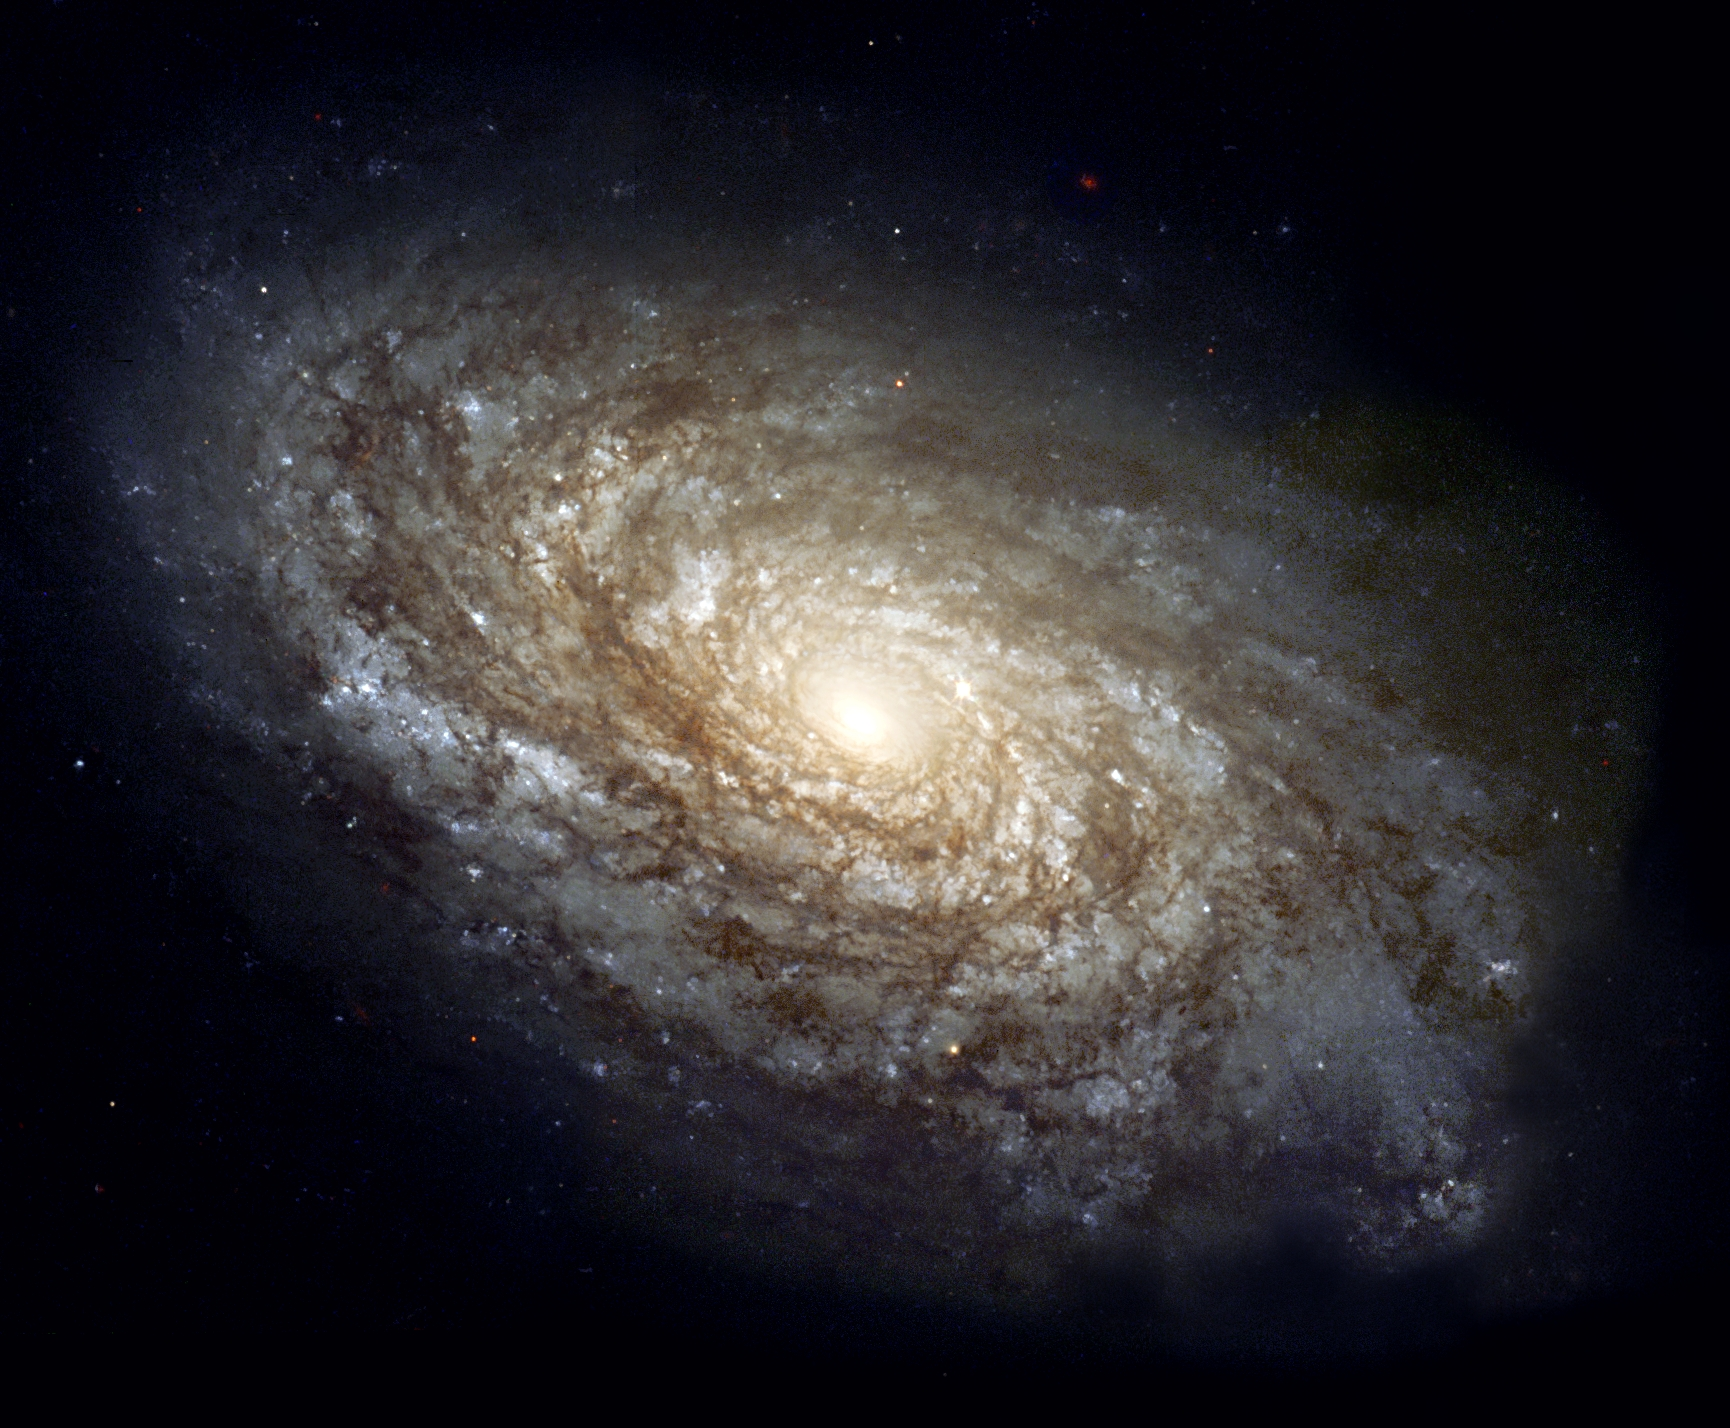
\includegraphics[width=0.67\textwidth]{figures/galaxy.jpg}
    \caption{Image of a galaxy.}
    \label{fig:galaxy}
\end{figure}

The quick brown fox jumped over the lazy dog. Here is \textbf{Table \ref{tab:words}}:

\begin{table}[H]
    \centering
    \caption{A table of words.}
    \label{tab:words}
    \begin{tabular}{l l l}
        \toprule
        \textbf{Foxtrot} & \textbf{Golf} & \textbf{Hotel} \\
        \midrule
        India & Juliett & Kilo     \\
        Lima  & Mike    & November \\
        Oscar & Papa    & Quebec \\
        \bottomrule
    \end{tabular}
\end{table}

Using \texttt{biblatex} you can display bibliography divided into sections,
depending of citation type. For example: Einstein's journal paper \cite{einstein} and the Dirac's book \cite{dirac} are physics related items.

\clearpage

\printbibliography[heading=bibintoc]
\clearpage

\begin{appendices}

\section{Romeo}
\lipsum[1-3]  % Filler text command

\clearpage

\section{Sierra}
\lipsum[4-6]

\clearpage

\end{appendices}

\end{document}
